% questions.tex —— 1988 年·广东卷·理工农医类 · 题目内容片段（无答案）
% 由 tools/generate_projects.py 依来源总账自 1988/1988_数学真题_广东理_试题.md 生成，勿手改（改源 MD 后重跑）


\gkpart{试题}

\begin{gktip}
\textbf{来源说明}：本题面依据固定源 PDF《1988 年全国普通高等学校招生统一考试广东省数学（理工农医类）》逐题转录。固定源共 9 页，PDF 第 1—4 页为题面，第 5—9 页为答案与解答。

\textbf{版式与异文说明}：固定源含文字层，但部分旧字体在抽取时会显示为私有字形，按页面视觉关系恢复为数学运算符。第 1 题第 23 小题题面写有“如右图”，但固定源 9 页中未见对应图形，保留题干并标记为缺图；第 1 题第 24 小题的 $\sin 10$、$\cos 5$ 按固定源原样记录，不擅自补加度数符号。

\textbf{图形说明}：第二卷第二题的四棱锥图依据固定源关系重绘为 TikZ 矢量图；第 1 题第 23 小题因固定源缺图不补画。
\end{gktip}

\begin{question}
\gkti{1}

第一卷满分 50 分，共有 25 个选择题。每题都给出代号为 A、B、C、D 的四个结论，其中只有一个结论正确。每题选对得 2 分，不选、选错或者选出的代号超过一个，一律得 0 分。

（1） 直线 $3x-2y=6$ 在 $y$ 轴上的截距是\mbox{（　　）}

（A）$\dfrac32$　　（B）$-2$　　（C）$-3$　　（D）$3$

\Needspace{5\baselineskip}
（2） 对数方程

\nopagebreak[4]
\[
2\log_6x=1-\log_6 3
\]

的解是\mbox{（　　）}

（A）$\sqrt3$　　（B）$\sqrt2$　　（C）$\sqrt2$ 和 $-\sqrt2$　　（D）$\sqrt3$ 和 $\sqrt2$

（3） 如果用 $C\text{、}R$ 和 $I$ 分别表示复数集、实数集和纯虚数集，其中 $C$ 为全集，那么有\mbox{（　　）}

（A）$C=R\cup I$　　（B）$R\cap I=\{0\}$

（C）$\overline R=C\cap I$　　（D）$R\cap I=\varnothing$

（4） 在等差数列 $\{a_n\}$ 中，已知前 15 项之和 $S_{15}=90$，那么 $a_8=$\mbox{（　　）}

（A）$3$　　（B）$4$　　（C）$6$　　（D）$12$

（5） 如果 $\operatorname{tg}A+\operatorname{ctg}A=m$，那么 $\sin2A=$\mbox{（　　）}

（A）$\dfrac1m$　　（B）$\dfrac2m$　　（C）$2m$　　（D）$\dfrac1{m^2}$

（6） 设 $a\text{、}b$ 是异面直线，那么\mbox{（　　）}

（A）必然存在唯一的一个平面同时平行于直线 $a$ 和 $b$

（B）必然存在唯一的一个平面同时垂直于直线 $a$ 和 $b$

（C）过直线 $a$ 存在唯一的一个平面平行于直线 $b$

（D）过直线 $a$ 存在唯一的一个平面垂直于直线 $b$

\Needspace{5\baselineskip}
（7） 当 $a\ne0$ 时，方程

\nopagebreak[4]
\[
x^2+y^2+ax-ay=0
\]

所表示的图形\mbox{（　　）}

（A）关于 $x$ 轴对称　　（B）关于 $y$ 轴对称

（C）关于直线 $y-x=0$ 对称　　（D）关于直线 $y+x=0$ 对称

\Needspace{5\baselineskip}
（8） 设 $\theta$ 是第四象限的角，那么方程

\nopagebreak[4]
\[
(\sin\theta)x^2+y^2=\sin2\theta
\]

所表示的曲线是\mbox{（　　）}

（A）焦点在 $x$ 轴上的椭圆　　（B）焦点在 $y$ 轴上的椭圆

（C）焦点在 $x$ 轴上的双曲线　　（D）焦点在 $y$ 轴上的双曲线

\Needspace{5\baselineskip}
（9） 抛物线

\nopagebreak[4]
\[
y^2=4x-2
\]

的准线的方程是\mbox{（　　）}

（A）$x=-\dfrac12$　　（B）$x=\dfrac14$　　（C）$x=0$　　（D）$x=-1$

（10） 过抛物线 $y^2=4x$ 的焦点，作直线与此抛物线相交于两点 $P$ 和 $Q$，那么线段 $PQ$ 中点的轨迹的方程是\mbox{（　　）}

（A）$y^2=2x-1$　　（B）$y^2=2x-2$　　（C）$y^2=-2x+1$　　（D）$y^2=-2x+2$

（11） 设正方体的全面积为 $24\,\mathrm{cm}^2$，一个球内切于该正方体，那么，这个球的体积是\mbox{（　　）}

（A）$\dfrac43\pi\,\mathrm{cm}^3$　　（B）$\dfrac83\pi\,\mathrm{cm}^3$

（C）$\sqrt6\pi\,\mathrm{cm}^3$　　（D）$\dfrac{32}3\pi\,\mathrm{cm}^3$

（12） “平面 $\alpha$ 内有无穷多条直线都和直线 $l$ 平行”是“$l\parallel\alpha$”的\mbox{（　　）}

（A）充分而不必要的条件　　（B）必要而不充分的条件

（C）必要且充分的条件　　（D）既不充分又不必要的条件

（13） 下列函数中，在区间 $(0,1)$ 上是增函数的只有\mbox{（　　）}

（A）$y=-\sqrt{x}$　　（B）$y=\dfrac1{x^3}$　　（C）$y=\log_{\frac12}x$　　（D）$y=-x^2+2x+1$

\Needspace{5\baselineskip}
（14） 下列不等式中，与不等式

\nopagebreak[4]
\[
\frac{x-3}{2-x}\geq0
\]

同解的是\mbox{（　　）}

（A）$(x-3)(2-x)\geq0$　　（B）$\lg(x-2)\leq0$

（C）$\dfrac{2-x}{x-3}\geq0$　　（D）$(x-3)(2-x)>0$

（15） 用 $0\text{、}1\text{、}2\text{、}3\text{、}4$ 这五个数字组成没有重复数字的四位数，那么，在这些四位数中，是偶数的总共有\mbox{（　　）}

（A）120 个　　（B）96 个　　（C）60 个　　（D）36 个

\Needspace{5\baselineskip}
（16） 如果

\nopagebreak[4]
\[
\operatorname{tg}(\alpha+\beta)=\frac25,
\qquad \operatorname{tg}\left(\beta-\frac\pi4\right)=\frac14,
\]

\Needspace{5\baselineskip}
那么

\nopagebreak[4]
\[
\operatorname{tg}\left(\alpha+\frac\pi4\right)=
\]

\mbox{（　　）}

（A）$\dfrac{13}{18}$　　（B）$\dfrac{13}{22}$　　（C）$\dfrac3{22}$　　（D）$\dfrac3{18}$

（17） 函数值 $\operatorname{tg}224^\circ\text{、}\sin136^\circ\text{、}\cos310^\circ$ 的大小关系是\mbox{（　　）}

（A）$\operatorname{tg}224^\circ<\sin136^\circ<\cos310^\circ$

（B）$\sin136^\circ<\cos310^\circ<\operatorname{tg}224^\circ$

（C）$\cos310^\circ<\operatorname{tg}224^\circ<\sin136^\circ$

（D）$\cos310^\circ<\sin136^\circ<\operatorname{tg}224^\circ$

（18） 如果椭圆的两个焦点将长轴分成三等分，那么这个椭圆的两条准线间的距离是焦距的\mbox{（　　）}

（A）18 倍　　（B）12 倍　　（C）9 倍　　（D）4 倍

（19） 记函数 $y=\dfrac1x$ 的图象为 $l_1$，$y=\operatorname{arctg} x$ 的图象为 $l_2$，那么 $l_1$ 与 $l_2$ 的交点个数是\mbox{（　　）}

（A）无穷多个　　（B）2 个　　（C）1 个　　（D）0 个

（20） 如果实数 $x\text{、}y$ 满足 $x^2+y^2=1$，那么 $(1-xy)(1+xy)$ 有\mbox{（　　）}

（A）最小值 $\dfrac12$ 和最大值 1　　（B）最大值 1 和最小值 $\dfrac34$

（C）最小值 $\dfrac34$ 而无最大值　　（D）最大值 1 而无最小值

\Needspace{5\baselineskip}
（21） 曲线

\nopagebreak[4]
\[
y=1+\sqrt{4-x^2}\qquad(-2\leq x\leq2)
\]

与直线 $y=k(x-2)+4$ 有两个交点时，实数 $k$ 的取值范围是\mbox{（　　）}

（A）$\left(\dfrac5{12},\dfrac34\right]$　　（B）$\left(\dfrac5{12},+\infty\right)$

（C）$\left(\dfrac13,\dfrac34\right]$　　（D）$\left(0,\dfrac5{12}\right)$

\Needspace{5\baselineskip}
（22） 设 $f(x)$ 是 $R$ 上的奇函数，且当 $x\in[0,+\infty)$ 时，

\nopagebreak[4]
\[
f(x)=x(1+\sqrt[3]{x}),
\]

那么 $x\in(-\infty,0)$ 时，$f(x)=$\mbox{（　　）}

（A）$-x(1+\sqrt[3]{x})$　　（B）$x(1+\sqrt[3]{x})$

（C）$-x(1-\sqrt[3]{x})$　　（D）$x(1-\sqrt[3]{x})$

（23） 已知 $y=f(x)$ 的图象如右图，那么 $f(x)=$\mbox{（　　）}

\begin{gktip}
\textbf{转录疑点}：固定源题面明确写“如右图”，但固定 PDF 第 1—4 页中未见该图形；以下四个选项按可见文字转录，不凭空补图。
\end{gktip}

（A）$\sqrt{x^2-2|x|+1}$　　（B）$x^2-2|x|+1$

（C）$|x^2-1|$　　（D）$\sqrt{x^2-2x+1}$

\Needspace{5\baselineskip}
（24）　

\nopagebreak[4]
\[
\sqrt{1+\sin10}=
\]

\mbox{（　　）}

\begin{gktip}
\textbf{转录疑点}：固定源选项中的 $\sin10$、$\cos5$ 没有度数符号，按原卷字面记录。
\end{gktip}

（A）$\cos5+\sin5$　　（B）$-\cos5-\sin5$　　（C）$\sqrt2\cos5$　　（D）$\cos5-\sin5$

（25） 一个三棱锥，如果它的底面是直角三角形，那么它的三个侧面\mbox{（　　）}

（A）必然都是非直角三角形　　（B）至多只能有一个是直角三角形

（C）至多只能有两个是直角三角形　　（D）可能都是直角三角形

\end{question}
\begin{question}
\gkti{2}

第二卷第一题（本题满分 15 分）共有 5 个小题，每小题满分 3 分。每个小题都有用横线表示的空位，请把你认为合适的内容写在横线上的空位里。

（1） 把极坐标方程 $\rho=4\sin\theta$ 化成直角坐标方程得　　　　。

（2） 函数 $y=|\cos x|$ 的最小正周期是　　　　。

（3） 复数 $-\sqrt6+\sqrt2i$ 的三角形式是　　　　。

\Needspace{5\baselineskip}
（4）　

\nopagebreak[4]
\[
\lim_{n\to\infty}
\frac{1-2+3-4+\cdots+(2n-1)-2n}{(n-1)\left(\frac1n+1\right)}
\]

的值是　　　　。

（5） 在 $(1+x+x^2)(1-x)^{10}$ 的展开式中，$x^5$ 的系数是　　　　。（用具体数字作答。）

\Needspace{0.4\textheight}
\end{question}
\begin{question}
\gkti{3}

第二卷第二题（本题满分 13 分）。如图，在四棱锥 $P-ABCD$ 中，侧面 $PCD$ 是边长为 $2\,\mathrm{cm}$ 的等边三角形，且与底面垂直，而底面 $ABCD$ 是面积为 $2\sqrt3\,\mathrm{cm}^2$ 的菱形，$\angle ADC$ 是锐角。
\nopagebreak[4]
\begin{center}% 1988 年广东卷理工农医类第二卷第二题：四棱锥 P-ABCD
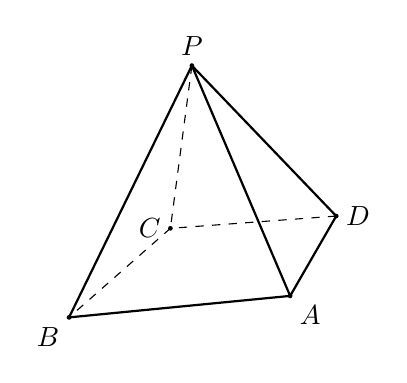
\begin{tikzpicture}[scale=0.78,>=stealth]
  \coordinate (P) at (2.0,4.1);
  \coordinate (B) at (0,0);
  \coordinate (A) at (3.6,0.35);
  \coordinate (D) at (4.35,1.65);
  \coordinate (C) at (1.65,1.45);
  \draw[thick] (P)--(B) (P)--(A) (P)--(D);
  \draw[dashed] (P)--(C);
  \draw[thick] (B)--(A)--(D);
  \draw[dashed] (D)--(C)--(B);
  \fill (P) circle (1.1pt) node[above] {$P$};
  \fill (A) circle (1.1pt) node[below right] {$A$};
  \fill (B) circle (1.1pt) node[below left] {$B$};
  \fill (C) circle (1.1pt) node[left] {$C$};
  \fill (D) circle (1.1pt) node[right] {$D$};
\end{tikzpicture}
\end{center}
\nopagebreak[4]
（1） 求这个四棱锥的体积。

（2） 求证：$PA\perp CD$。

\end{question}
\begin{question}
\gkti{4}

\Needspace{5\baselineskip}
第二卷第三题（本题满分 14 分）。已知双曲线的方程是

\nopagebreak[4]
\[
16x^2-9y^2=144.
\]

（1） 求这双曲线的焦点坐标、离心率和渐近线方程；

（2） 设 $F_1$ 和 $F_2$ 是这双曲线的左、右焦点，点 $P$ 在这双曲线上，且 $|PF_1|\cdot|PF_2|=32$，求 $\angle F_1PF_2$ 的大小。

\end{question}
\begin{question}
\gkti{5}

\Needspace{5\baselineskip}
第二卷第四题（本题满分 14 分）。设 $0<\theta<2\pi$，复数

\nopagebreak[4]
\[
z=1-\cos\theta+i\sin\theta,qquad u=a^2+ai,
\]

且 $zu$ 是纯虚数，这里 $i$ 是虚数单位，$a$ 是实数。

（1） 求复数 $u$ 的辐角主值 $\arg u$（用 $\theta$ 的代数式表示）；

（2） 记 $\omega=z^2+u^2+2zu$，试问：$\omega$ 可能是正实数吗？为什么？

\end{question}
\begin{question}
\gkti{6}

\Needspace{5\baselineskip}
第二卷第五题（本题满分 14 分）。设 $a>0$，$a\ne1$，

\nopagebreak[4]
\[
f(x)=\log_a\left(x+\sqrt{x^2-1}\right)\qquad(x\ge1).
\]

（1） 求函数 $f(x)$ 的反函数 $f^{-1}(x)$ 和这个反函数的定义域；

\Needspace{5\baselineskip}
（2） 记 $b_n=f^{-1}(n)$，$S_n=b_1+b_2+\cdots+b_n$，求证：当

\nopagebreak[4]
\[
\frac12<a<2
\]

\Needspace{5\baselineskip}
时，对任意自然数 $n$，都有

\nopagebreak[4]
\[
S_n<2^n-\left(\frac{\sqrt2}{2}\right)^n.
\]

\end{question}